\documentclass[../main]{subfiles}
\begin{document}
\setcounter{secnumdepth}{2}
    \chapter{提案手法}
        \section{全天球カメラに基づく通路認識手法}
        本研究は,全天球カメラで取得した画像に基づき通路認識を行う手法の検証を行う.
        そこで,\fref{figure::proposed_method_fig}に示すようなYOLOを用いた手法を提案する.
        本研究では,360度カメラの主要な画像形式である「エクイレクタングラー(equirectangular)」形式の全天球カメラ画像を用いる.
        また,全天球カメラにより得られた画像は,後方の通路が見切れており,学習後の精度確認の段階で通路の認識がうまくできていなかったため,
        \fref{figure::image_proc_fig}に示すような画像の前処理を施した.
        YOLOの学習モデル作成のため,自作のデータセットを作成し,学習を行う.画像データは,
        実験環境として想定している本学の津田沼キャンパス2号館3階で実験につかうロボットに
        全天球カメラを取り付けて収集した.データセットの一例を\fref{figure::dataset_fig}に示す.
        また,データセットのクラスは\tref{table::datasets_table}の11クラスで設定した.
        
        \begin{figure}[H]
        \centering
        \fbox{
        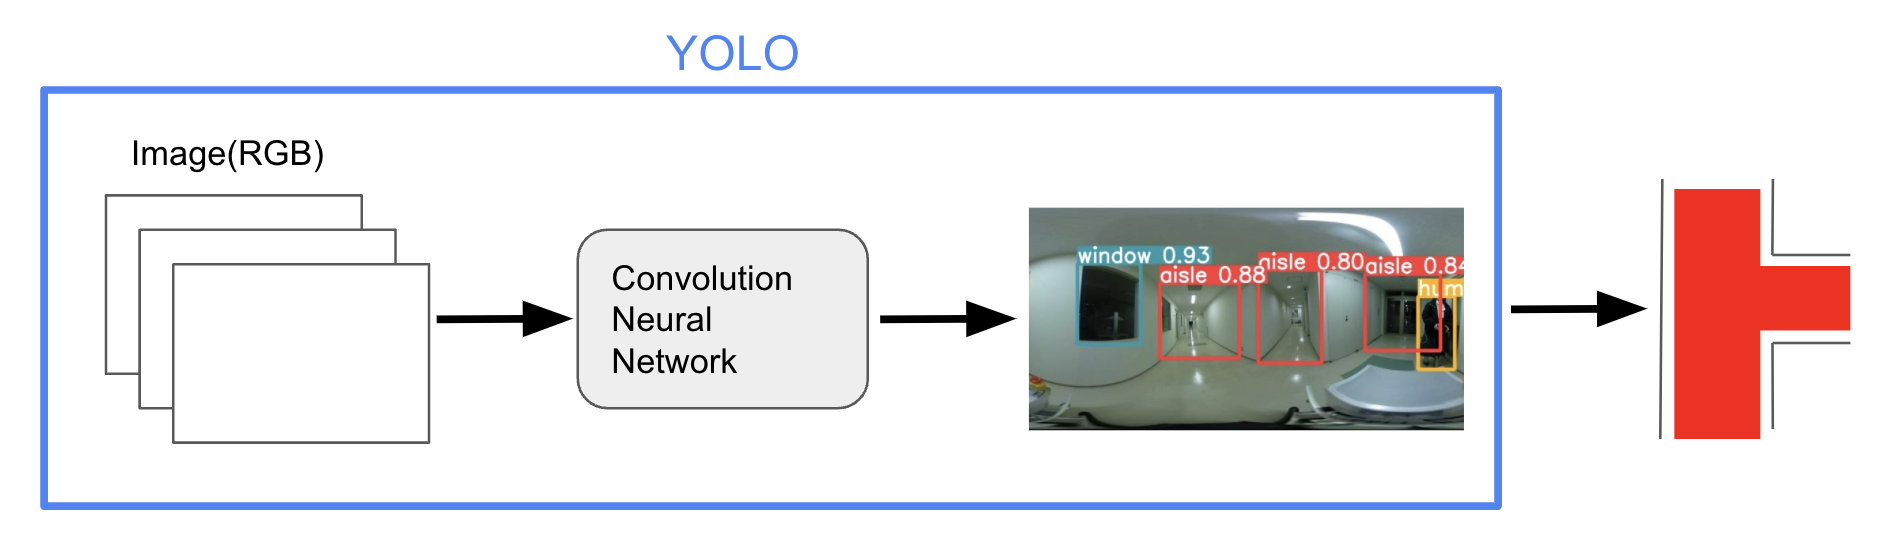
\includegraphics[width=10cm]{proposed_method2.png}
        }
        \caption{Flow of passage recognition method.}
        \label{figure::proposed_method_fig}
        
        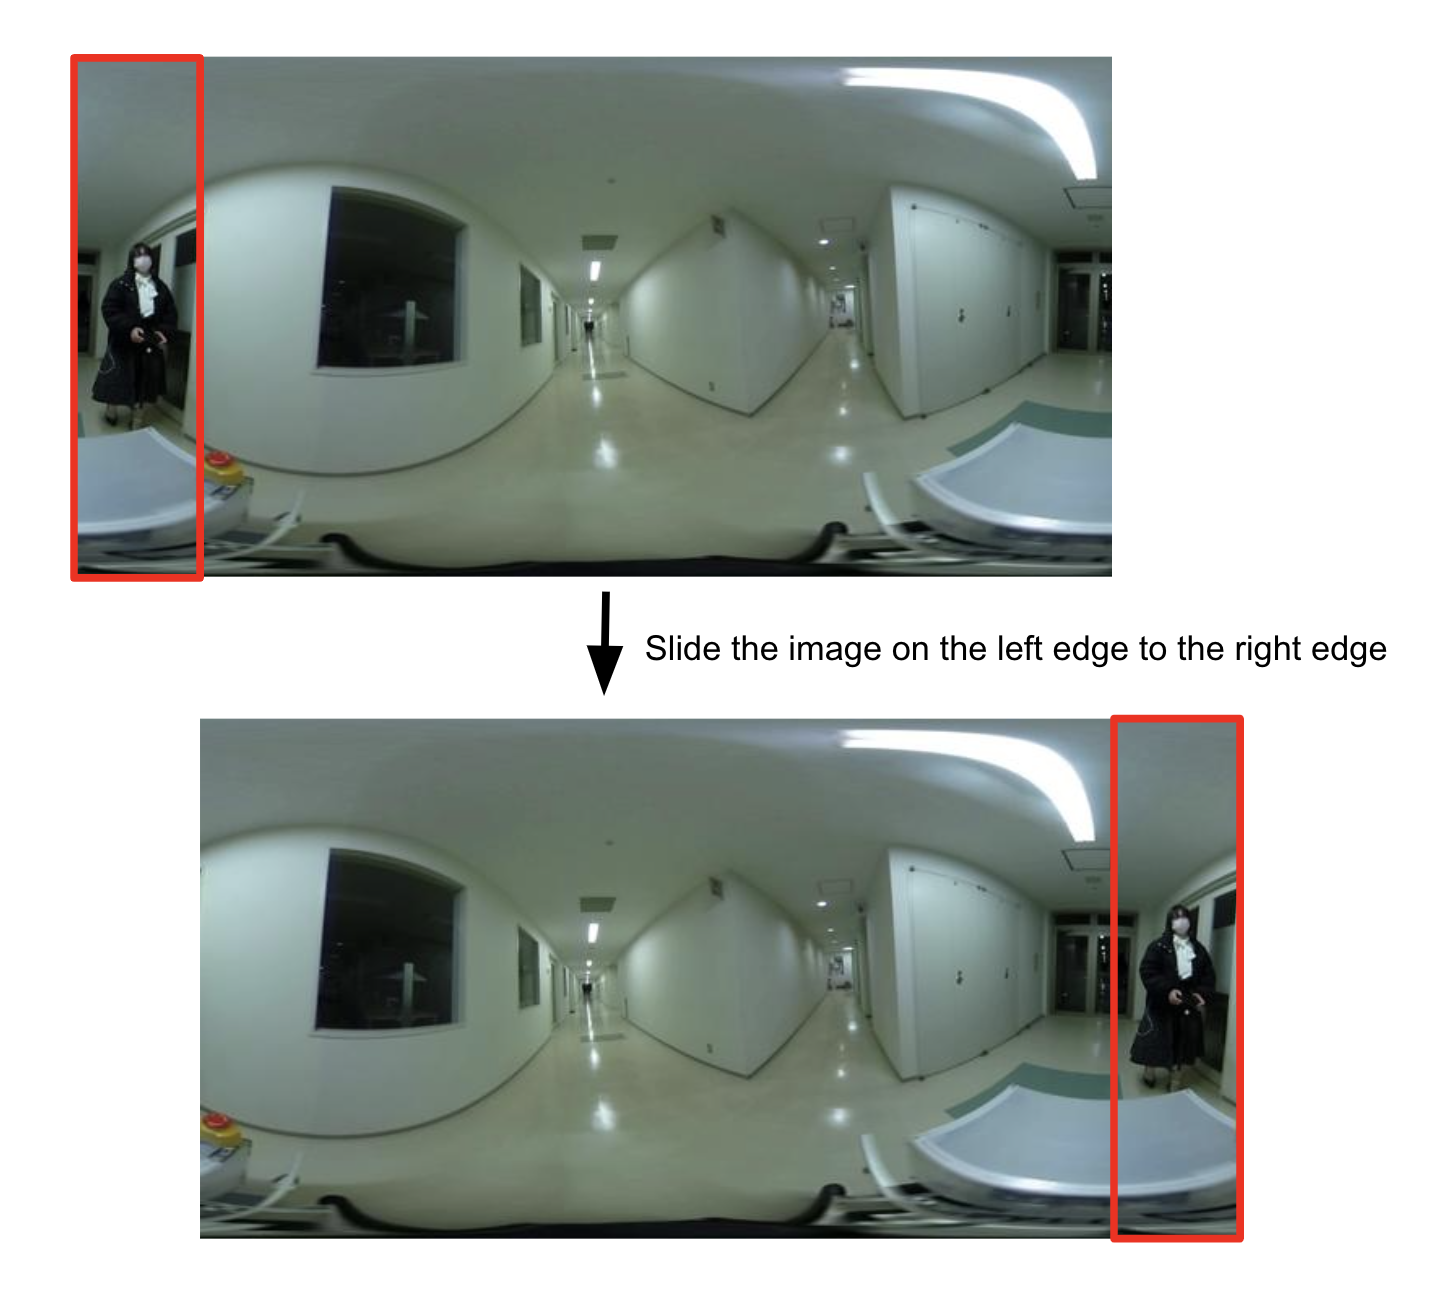
\includegraphics[width=10cm]{image_proc_exp.png}
        \caption{Preprocessing of spherical camera images.}
        \label{figure::image_proc_fig}
        
        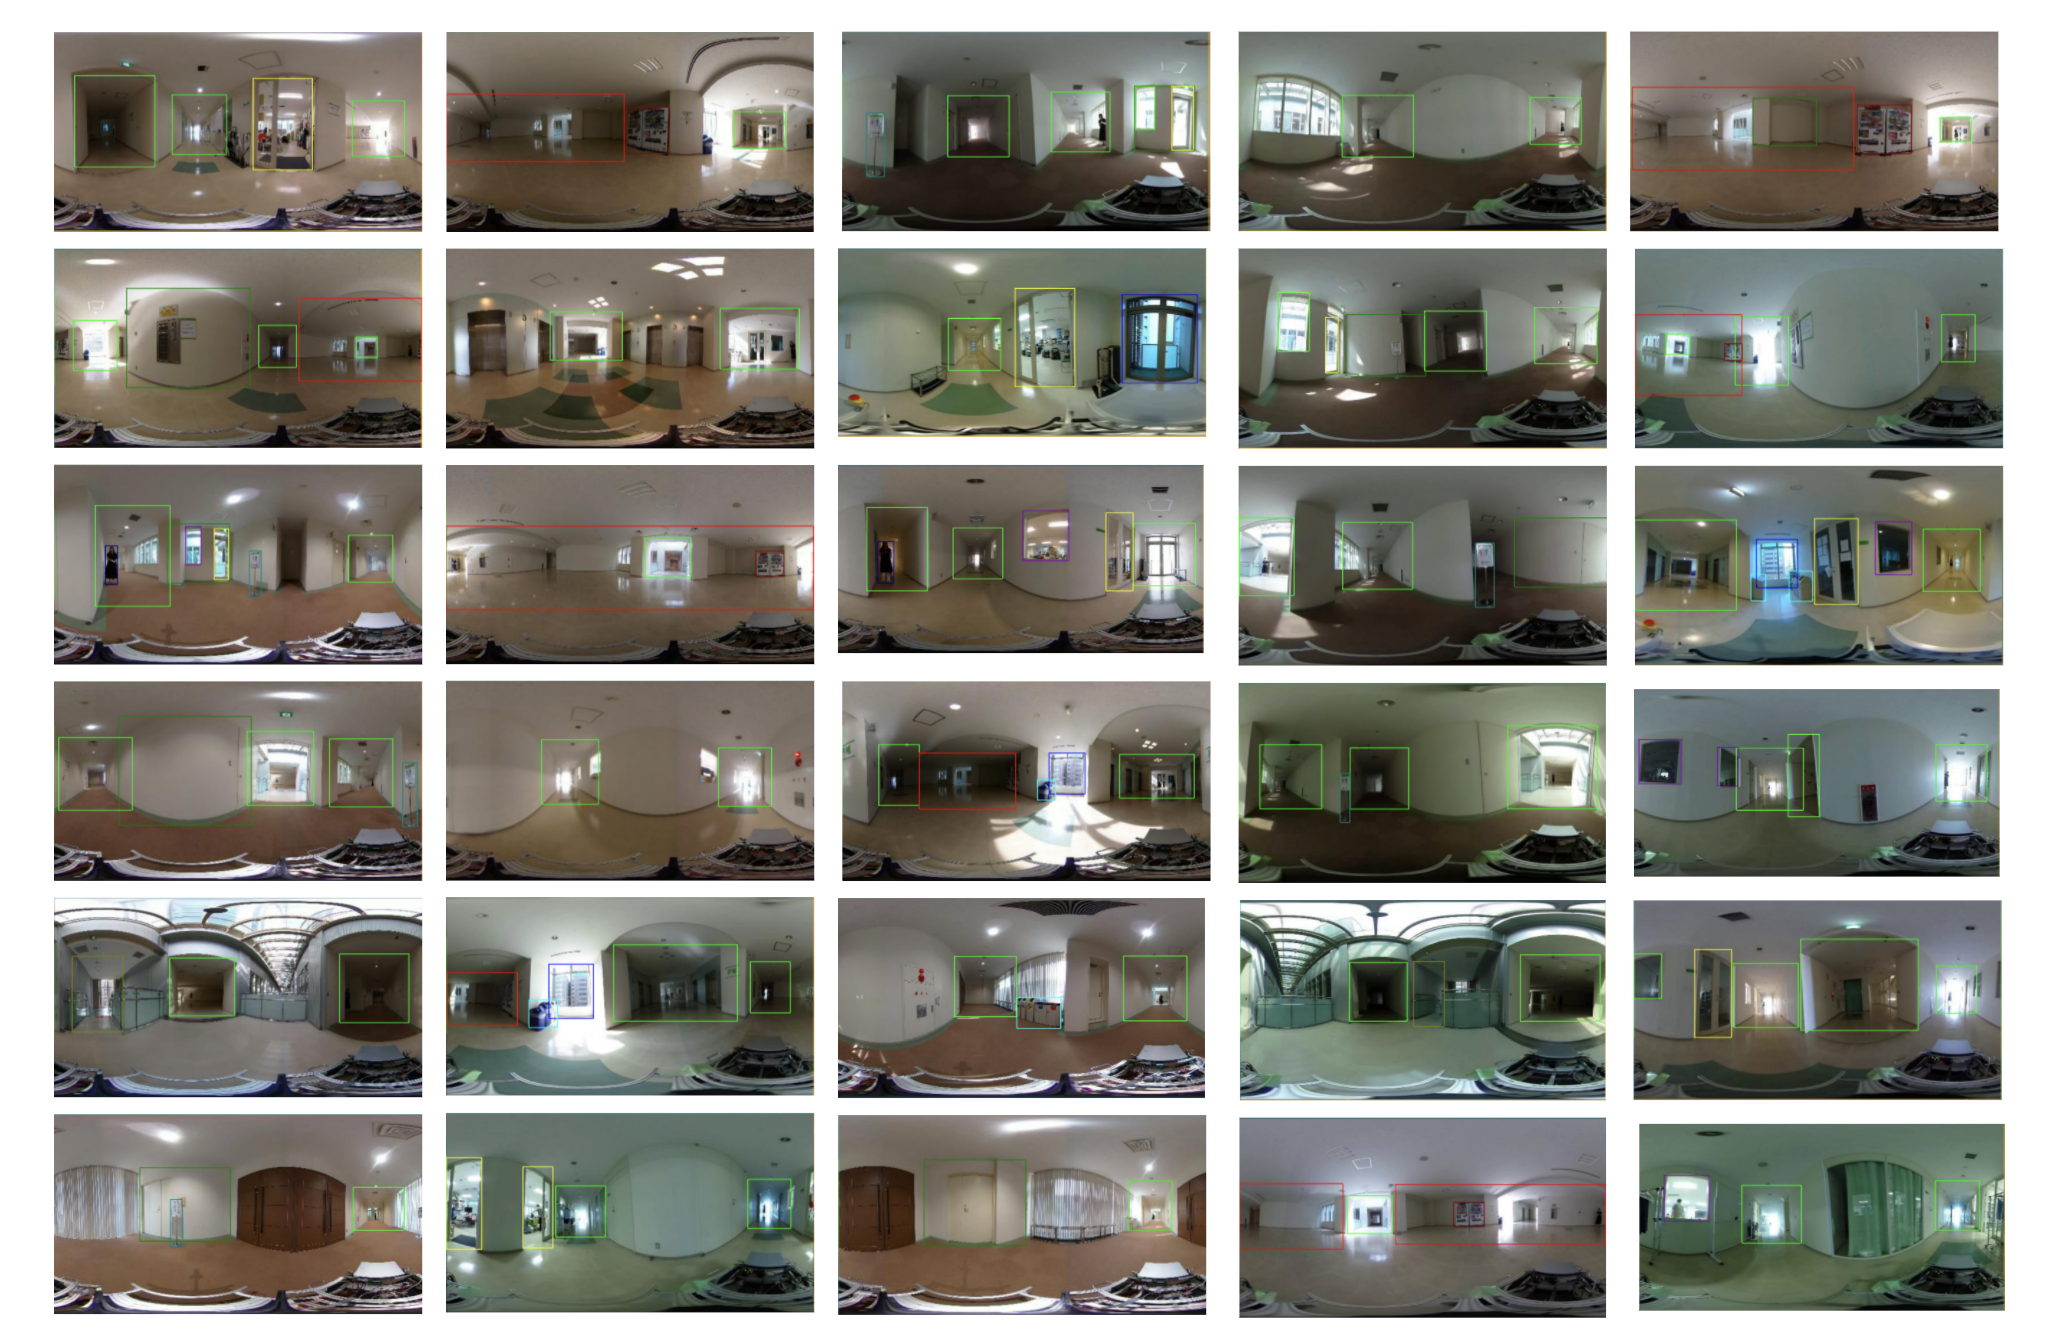
\includegraphics[width=15cm]{dataset_exp.png}
        \caption{An example of a dataset.}
        \label{figure::dataset_fig}


        \end{figure}

        \begin{table}[H]
            \caption{Class name to be labeled.}
            \centering
            \label{table::datasets_table}
            \begin{tabular}{lllll}
            \hline
            name of the class &  &  &  &  \\ 
            \hline \hline
            aisle             &  &  &  &  \\
            end               &  &  &  &  \\
            door\_end         &  &  &  &  \\
            human             &  &  &  &  \\
            door              &  &  &  &  \\
            step              &  &  &  &  \\
            square            &  &  &  &  \\
            vending\_machine  &  &  &  &  \\
            trash\_can        &  &  &  &  \\
            signboard         &  &  &  &  \\
            window            &  &  &  &  \\ 
            \hline
            \end{tabular}
        \end{table}
\end{document}